\documentclass{article}
\usepackage{graphicx}
\usepackage{blindtext}
\usepackage[T1]{fontenc}
\usepackage[utf8]{inputenc}
\usepackage{mathtools}
\usepackage{amssymb}
\usepackage{amsmath}
\usepackage{gensymb}
\usepackage{url}
\usepackage{float}
\usepackage{fancyhdr}
\usepackage[a4paper,left=3cm,right=3cm,top=2cm,bottom=4cm,bindingoffset=5mm]{geometry}
\usepackage{etoolbox}%
\usepackage[ngerman]{babel}

\newcommand{\makefootnotelist}[1]{%
	\parbox{0.8\textwidth} {%
		\footnotesize{%
			\renewcommand*{\do}[1]{##1\\}%
			\dolistcsloop{#1}}}}%
\newcommand{\fancyfootnote}[1]{%
	\footnotemark{}%
	\def\listname{footlist\thepage}%
	\def\n{$^{\the\numexpr\value{footnote}}$}
	\ifcsdef{\listname}%
	{\listcseadd{\listname}{\n\ #1}}%
	{\csedef{\listname}{}%
		\listcseadd{\listname}{\n\ #1}}%
	\fancypagestyle{fancyfootnote}{%
		\fancyfoot[LO,RE]{\makefootnotelist{\listname}}%
		\fancyfoot[RO,LE]{Page \thepage}%
		\fancyfoot[C]{}%
	}\thispagestyle{fancyfootnote}}%


\pagestyle{fancy}
\fancyhf{}
\rhead{\leftmark}
\lhead{B3.1}
\rfoot{Page \thepage}
\renewcommand{\footrulewidth}{0.2pt}


\title{Praktikumsbericht B 3.1: \\ \underline{Statistik der Kernzerfälle}}
\author{Alexander Obradovic\\
		\texttt{7338968}
		\and
		Marcus Sickmöller\\
		\texttt{7359786}
		\and
		Tom Sittig\\
		\texttt{7345424}}
\date{07.05.2021}

\begin{document}
	\maketitle
	\begin{center}
	
\includegraphics[scale=0.13]{siegel.jpg}
	\end{center}
	
	\newpage
	\tableofcontents
	\newpage
	\section{Einführung}
	In diesem Versuch wollen wir uns mit der grundlegenden Statistik von Kernzerfällen vertraut machen. Dazu wird bei drei verschiedenen Spannungen die emittierte Strahlung von Kernzerfällen mittels eines Zählrohrs gemessen und diese Daten dann statistisch ausgewertet. \\
	Die theoretische Vorbereitung beschäftigt sich mit den Grundlagen der Statistik sowie der Funktionsweise des Zählrohrs. Dadurch wurde die Basis für die Auswertung der Versuchsdaten erarbeitet. \\
	In der Auswertung werden zunächst Poisson sowie Gauß-Verteilungen aus den Messdaten extrahiert, die Intervall-Verteilung mit einer theoretischen Funktion verglichen sowie verschiedene Hypothesen zum $\chi^2$-Test überprüft. Zuletzt wird noch die Totzeit des Zählrohrs mithilfe der Zwei-Präparat-Methode bestimmt. \\\\
	Aufgrund der aktuellen Pandemiesituation war es uns nicht möglich, die Messungen vor Ort selbst durchzuführen, der Fokus dieses Versuchsprotokolls liegt also auf einer gründlichen theoretischen Vorbereitung und der Auswertung der uns zur Verfügung gestellten Messdaten.
	\section{Vorbereitung}
	\subsection{Halbwertszeit von $^{137}$Cs}
	In dem Versuchsaufbau werden zwei Caesium 137 Quellen verwendet, welches ein Radioaktives Isotop mit einer Halbwertszeit von $30.05a$\fancyfootnote{W.M. Haynes, CRC Handbook of Chemistry and Physics (97th Edition, 2016), Kpt. 11-77} ist.
	\subsection{Wahrscheinlichkeitsfunktion, -dichte, -verteilung}
	Gegeben einer Zufallsvariable $X$, welche Element einer Menge möglicher Ereignisse $M\subseteq\mathbb{R}$ sei, ist eine \textbf{Wahrscheinlichkeitsverteilung} jene Funktion $F(x)$, die angibt, mit welcher Wahrscheinlichkeit die Zufallsvariable einen Wert $\leq x$ annimmt. Hierbei unterscheidet sich $F(x)$ danach, ob $M$ diskret oder überabzählbar ist.\\\\
	Bei diskreter Menge ist die Wahrscheinlichkeitsverteilung $F(x)$ gegeben als\\
	\begin{gather}
	F(x)=\sum_{x_i\leq x}f(x_i),
	\end{gather}
	wobei $f(x)$ die \textbf{Wahrscheinlichkeitsfunktion} ist, welche für jeden diskreten Wert $x$ eine Eintrittswahrscheinlichkeit annimmt.\\\\
	Ist die Menge $M$ überabzählbar, so ist die Wahrscheinlichkeit, das ein bestimmtes Ereignis eintritt $0$. Um $F(x)$ nun zu erhalten wird über die kontinuierliche \textbf{Wahrscheinlichkeitsdichte} $f(y)$ integriert
	\begin{gather}
	F(x)=\int_{-\infty}^{x}f(y)dy
	\end{gather}   
	\subsection{Verteilungen}
	\subsubsection{Binomial}
	Für ein Zufallsexperiment mit zwei möglichen, diskreten, exklusiven, Ereignissen $A,B$ mit den Eintrittswahrscheinlichkeiten 
	\begin{equation}
	P(A)=p,\qquad P(B)=q=1-p
	\end{equation}
	ist bei $N$ unabhängigen Durchführungen die Gesamtwahrscheinlichkeit des Eintretens von $n\cdot A$ und $(N-n)\cdot B$ Ereignissen in einer bestimmten, aber beliebigen, Reihenfolge 
	\begin{equation}
	p^n\cdot(1-p)^{N-n}.
	\end{equation}
	Das Eintreten von $n\cdot A$ und $(N-n)\cdot B$ Ereignissen über alle möglichen Reihenfolge in der diese Eintreten können ist mithilfe des Binomialkoeffizienten gegeben als
	\begin{equation}
	P(N,n,p)=\binom{N}{n}p^n(1-p)^{N-n}.
	\end{equation}
	Dieser besitzt einen Erwartungswert $m=Np$ und eine Varianz $\sigma^2=Np(1-p)$.
	\subsubsection{Poisson}
	Die Poissonverteilung ist eine Grenzverteilung für $N \rightarrow\infty,\quad p\rightarrow0$ mit der zusätzlichen Bedingung $Np=\lambda=const.$, also eine diskrete Verteilung bei einer sehr großen Anzahl an Zufallswerten. Die Wahrscheinlichkeitsfunktion
	\begin{equation}
	P(n,\lambda)=\frac{\lambda^n e^{-\lambda}}{n!}
	\end{equation}
	ergibt sich auf dem Limes der Binomialverteilung für $N\rightarrow\infty$.
	\subsubsection{Gauß}
	Die Gaußverteilung, mit Mittelwert $\mu$ und Varianz $\sigma^2$ 
	\begin{equation}
	P(x,\mu,\sigma)=\frac{1}{\sqrt{2\pi}\sigma}e^{-\frac{1}{2}\left(\frac{x-\mu}{\sigma}\right)^2}
	\end{equation}
	Ist eine kontinuierliche Wahrscheinlichkeitsfunktion. Sowohl Poisson-, als auch Binomialverteilung konvergieren gegen einen Spezialfall der Gaußverteilung mit $\mu=0,\;\sigma^2=1$ (die Normalverteilung) unter folgenden Bedingungen: Die Poissonverteilung, wenn $\lambda\gg1$ und die Binomialverteilung, wenn $N\rightarrow\infty,\;0<p<1$.
	\subsection{Varianz}
	Die Varianz $\sigma^2$ ist das Quadrat der Standardabweichung $\sigma$ und somit definiert als die mittlere quadratische Abweichung einer Zufallsvariable $X$ von einem Mittelwert $\mu$ der jeweiligen Verteilung.\\
	Die Varianz beschreibt somit, wie dicht die einzelnen Ergebnisse an ihrem Mittelwert liegen, bei kleinerem $\sigma^2$ ist der Peak der Verteilung schärfer, bei größerem breiter.\\
	Ein stärkere Relation besteht, falls die Zufallsvariablen $X={x_1,...,x_n}$ diskret und mit gleicher Wahrscheinlichkeit $p_i=p=\frac{1}{n}$ eintreten. Dann gilt
	\begin{gather}
	\mu=\frac{1}{n}\sum_{i=1}^{n}x_i=\bar{x}\\
	\sigma^2=\frac{1}{n}\sum_{i=1}^{n}(x_i-\bar{x})^2=\frac{1}{n}\sum_{i=1}^{n}(x_i-\mu)^2
	\end{gather} 
	\subsection{Intervallverteilung}
	Die Intervallverteilung beschreibt die Wahrscheinlichkeit, mit der ein Zeitintervall zwischen dem Eintreten zweier Ereignisse die Länge t besitzt.\\
	In dem Fall unseres Versuches hat dies also praktische Verwendung zur Beschreibung der Zeitintervalle zwischen den Zerfällen zweier instabiler Isotope.\\
	Die Intervallverteilung setzt sich zusammen als das Produkt zweier Einzelwahrscheinlichkeiten:\\\\
	Das kein Zerfall während eines gegebenen Zeitfensters stattfindet $W_1=e^{-\lambda}$, was der Poissonverteilung mit $n=0$ entspricht.\\
	$W_2=a\cdot dt$ der Wahrscheinlichkeit das in der Zeit $dt$ danach ein Zerfall stattfindet, wobei $a$ die Zerfallswahrscheinlichkeit des Materials ist.\\\\
	Das Produkt ist somit die Wahrscheinlichkeit
	\begin{equation}
	W=ae^{-\lambda}dt
	\end{equation}
	Die Wahrscheinlichkeitsdichte ergibt sich als die Ableitung von $W$ und es besteht zudem der Zusammenhang $\lambda=at$.
	\begin{equation}
	P(t)=ae^{-at}
	\end{equation}
	diesen Ausdruck kann man nun verallgemeinern auf ein Intervall in dem über ein gegebenes $t$ nur $n$ Zerfälle stattfinden, die Intervallverteilung.
	\begin{equation}
	P_n(t)=a\frac{(at)^n}{n!}e^{-at}
	\end{equation} 
	Besonders anschaulich werden diese Wahrscheinlichkeitsdichten graphisch aufgetragen, hier mit $a=1$ gegen arbiträre Zeiteinheiten:
	\begin{center}
	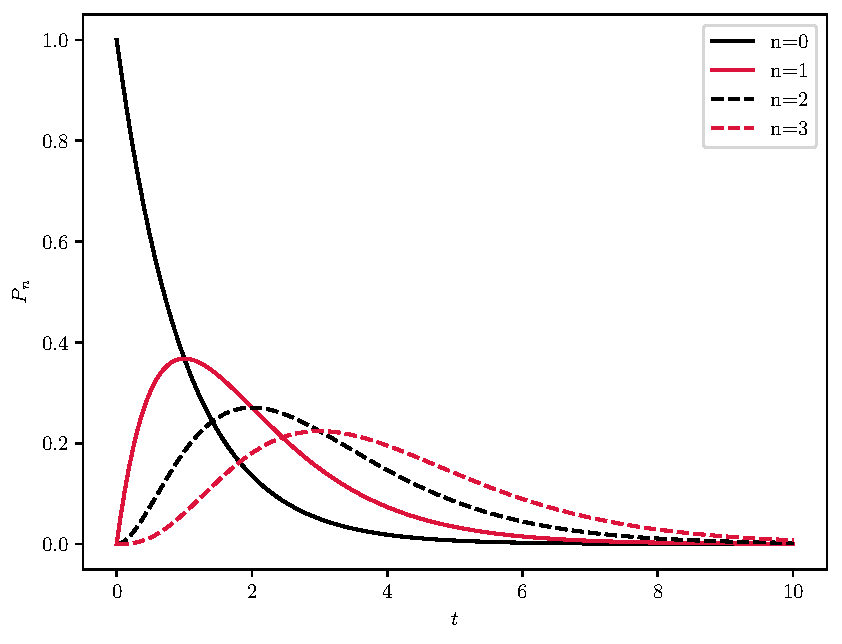
\includegraphics[scale=0.8]{Intervallverteilung.pdf}
	\end{center} 
	\subsection{Zusammenhang Verteilungen und Kernzerfall}
	Die Wahrscheinlichkeit $\omega$ mit der ein Isotop über einen Zeitraum $\Delta t$ zerfällt ergibt sich mithilfe der Zerfallswahrscheinlichkeit $\alpha$, einer für jedes Isotop charakteristische Konstante, wenn $\Delta t$ viel kleiner als die Halbwertszeit.\\
	Man kann die Zeitspanne $\Delta t$ der Zerfallswahrscheinlichkeit sowie die ihres Reziprokens in $k$ Abschnitte unterteilen und mit $\lim_{k \rightarrow\infty}$ erhält man somit die Wahrscheinlichkeit
	\begin{equation}
	\omega(t)=1-e^{-\alpha t}.
	\end{equation}  
	Mit der Halbwertszeit kann durch einsetzten $\alpha$ berechnet werden, als 
	\begin{equation}
	\omega(T_{1/2})=\frac{1}{2} \Leftrightarrow \alpha=-\frac{ln(\frac{1}{2})}{T_{1/2}}
	\end{equation}
	\newpage \noindent
	Da in praktischen Experimenten mit mehr als einen Kern gearbeitet wird ist es sinnvoll eine Zerfallswahrscheinlichkeit für $n$ Kerne über eine Zeitspanne zu berechnen, welche eine Binomialverteilung ist.
	\begin{gather}
	\omega(n,N,t)=\binom{N}{n}(1-e^{\alpha t})^ne^{-\alpha(N-n)t}\\
	\text{mit }p\equiv1-e^{-\alpha t} \Leftrightarrow P(N,n,p)=\binom{N}{n}p^n(1-p)^{N-n}
	\end{gather} 
	\subsection{Geiger-Müller-Zählrohr}
	Für den Nachweis ionisierender Strahlung mit einer Ionisationskammer wird aufgrund des sehr kleinen Ionisationsstroms ein Messverstärker benötigt. Eine solche Messung ist sehr empfindlich gegenüber Umwelteinflüssen. Schon das Annähern des Experimentators kann den Ausschlag verändern.\\
	Das Geiger-Müller-Zählrohr (GMZ) ist hingegen ein sehr robustes Nachweisgerät für radioaktive Strahlung. \\
	Ein Zählrohr kann, abhängig von der Versorgungsspannung, in verschiedenen Bereichen betrieben werden. Hier beschrieben ist nur den Geiger-Müller-Bereich (Auslösebereich).
	\begin{itemize}
	\item Zwischen dem positiv geladenen Zähldraht und dem negativ Zählrohrmantel herrscht ein zylindersymmetrisches elektrisches Feld, das um den Zähldraht am stärksten ist (höchste Feldliniendichte um den Draht).
	\item Die radioaktive Strahlung erzeugt auf dem Weg durch das Füllgas Elektron-Ion-Paare.
	\item Die Ionen bewegen sich (langsam) zum Zählrohrmantel, die Elektronen werden zum Zähldraht hin stark beschleunigt und bilden dabei ihrerseits weitere Elektron-Ion-Paare. Es kommt zur Ausbildung einer Elektronenlawine, die sich auf den Zähldraht zu bewegt.
	\item Bei der Wechselwirkung der Elektronen mit den Atomen des Füllgases kommt es im Auslösebereich auch zur Bildung von Photonen, die ihrerseits neue Ladungspaare bilden.
	\item Das ganze Zählrohr wird von einer Entladung erfasst. Der fließende Strom verursacht am Widerstand R einen Spannungsimpuls, der vom Zähler registriert wird.
	\item Im Auslösebereich ist die gebildete Ladungsmenge unabhängig von der Primärionisation, d.h. jedes radioaktive Teilchen löst eine Entladung aus.
	\end{itemize}
	\subsection{Totzeit}
	Unmittelbar nach einem Impuls ist das Zählrohr für eine kurze Zeit, die sog. Totzeit, für neu einfallende ionisierende Strahlung völlig unempfindlich. Die Totzeit beträgt bei den üblichen Zählrohren 10-4 bis 10-5 s. Danach sind für eine weitere Zeit die Impulshöhen kleiner und erreichen erst allmählich die Ausgangshöhe
	\subsubsection{Zwei Präparate Methode}
	Man misst unter gleichen Bedingungen die Impulsrate $I'_1$ einer Quelle 1, die Impulsrate $I'_2$ einer Quelle 2 und schließlich die Impulsrate $I'_{1,2}$ beider Quellen zusammen. Daraus lässt sich die Totzeit folgendermaßen berechnen\\
	\begin{equation}
	\tau'=\frac{1}{I'_{1,2}}-\frac{\sqrt{I'_1I'_2(I'_{1,2}-I'_1)(I'_{1,2}-I'_2)}}{I'_1I'_2I'_{1,2}}
	\end{equation}
	\subsubsection{Gemessene Zählraten}
	Die gemessene Zählrate $a'$ ist kleiner als die tatsächliche Zählrate $a$. Für jedes detektierte Teilchen muss man also nur $a\tau$ Teilchen dazu zählen. Dadurch ergibt sich nach Umformen:
	\begin{equation}
	a=\frac{a'}{1-a'\tau}
	\end{equation} 
	\subsubsection{Gemessene Verteilung}
	Wenn die Messwerte aus einer Poissonverteilung stammen, dann gilt außerdem $\sigma^2=m$ und die Verteilung besitzt die gleiche relative Breite wie die ursprüngliche.
	\begin{equation}
	\frac{\sigma}{m}=\frac{\sigma'}{m'}=\frac{1}{\sqrt{m}}
	\end{equation}
	Insgesamt folgt also:
	\begin{equation}
	\sigma'^2=m'\c(1-\tau a')
	\end{equation}
	\begin{equation}
	\sigma^2=\sigma'^2\cdot\left(\frac{a}{a'}\right)^2=\frac{m'}{1-\tau a}=m
	\end{equation}
	\subsection{$\chi^2$-Test}
	Die $\chi^2$-Verteilung beschreibt quadrierte Zufallsvariable einer Standardnormalverteilung. Sie wird auch $\chi^2$-Verteilung mit einem Freiheitsgrad genannt. Weitere Zufallsvariablen werden quadriert und zur vorherigen addiert. Bei n-Zufallsvariablen erhalten wir eine $\chi^2$-Verteilung mit n Freiheitsgraden.\\
	Die Idee beim $\chi^2$-Test, ist es eine bestimmte Verteilung als Hypothese anzunehmen. Diese hat einen Mittelwert $x$ und eine Varianz $y$. Wenn wir nun bei Experimenten Messwerte erhalten, die weit außerhalb der Varianz um den Mittelwert liegen können wir die Hypothese verwerfen. Sind die Messwerte jedoch um den Mittelwert im Bereich der Varianz gegeben so können wir sagen, dass unsere Hypothese stimmen könnte, aber wir können dies nicht mit $100 \%$-iger Sicherheit feststellen, sowie wir auch eine Irrtumswahrscheinlichkeit größer null haben, wenn wir etwas verwerfen.\\
	Wir können uns eine Ablehnungsvorraussetzung definieren, in dem wir uns eine feste Irrtumswahrscheinlichkeit vorgeben und diese dann auf die Dichtefunktion der $\chi^2$-Verteilung anwendet. Wir können jedoch keine Hypothese als „die richtige“ annehmen, da wir niemals alle bis auf eine Hypothese ohne Irrtumswahrscheinlichkeit verwerfen können.\\
	Ein kleines $\chi^2$ bedeutet nicht, dass die Daten gut zu der Hypothese passen, sondern dass sie sehr nah am Mittelwert liegen. Jedoch wollen wir erreichen, dass die Varianz der Verteilung der Hypothese entspricht. Wenn wir eine Gaußverteilung um 0 mit der Varianz 1 erreichen wollten, so müssen wir $\chi^2$ Werte die nah an 1 liegen annehmen aber welche die nah an der 0 liegen Verwerfen, da bei diesen die Varianz nicht der gewählten Verteilung entspricht. 
	Durch mehr Daten können wir die Hypothesen mit geringerer Irrtumswahrscheinlichkeit ausschließen und somit auch die Ablehnungsvorraussetzung schärfer auslegen. Aus den übrig gebliebenen Hypothesen kann man nun eine Verteilung bilden, die mit geringem Fehler den Messwerten entspricht.
	\newpage
	\section{Versuchsdurchführung}
	Wie bereits in der Einführung erläutert fand das Praktikum während der Covid-19 Pandemie, weshalb keine Messdatenerhebung vor Ort möglich war. Stattdessen wurden uns zuvor erhobene Messwerte zur Verfügung gestellt.\\
	Diese umfassen 3 Messungen über jeweils 45 Minuten von $^{137}Cs$ Quellen in den Anordnungen\\
	\begin{itemize}
	\item Quelle 7 bei 500 Volt
	\item Quelle 7 bei 600 Volt
	\item Quellen 6 \& 7 bei 500 Volt\\
	\end{itemize} 
	Die den Zeitpunkt jeder Zählung beinhalten.\\
	Sowie Messungen über 5 Minuten in den Anordnungen\\
	\begin{itemize}
	\item Quelle 6 bei 500, 600 \& 700 Volt
	\item Quelle 7 bei 500, 600 \& 700 Volt
	\item Quellen 6 \& 7 bei 500, 600 \& 700 Volt
	\item Untergrundmessung bei 500, 600 \& 700 Volt.\\
	\end{itemize}
	Der verwendete Versuchsaufbau bestand aus einem Geiger-Müller-Zählrohr, vor welches die zu betrachtende Probe platziert wird. An diesem liegt eine regulierbare Spannungquelle an.\\
	Das Geiger-Müller-Zählrohr gibt ein Rechtecksignal aus, wenn immer ein Event registriert wird, welches an den Computer weitergeleitet und von diesem ausgewertet wird.
	\newpage
	\section{Auswertung}
	\subsection{Poisson-Verteilung}
	\begin{center}
	\vfill
	\textbf{Abb. 1:}$\quad$Quelle 7 bei 500V: $\lambda=8.18\;,\sigma^2=3.90$	
	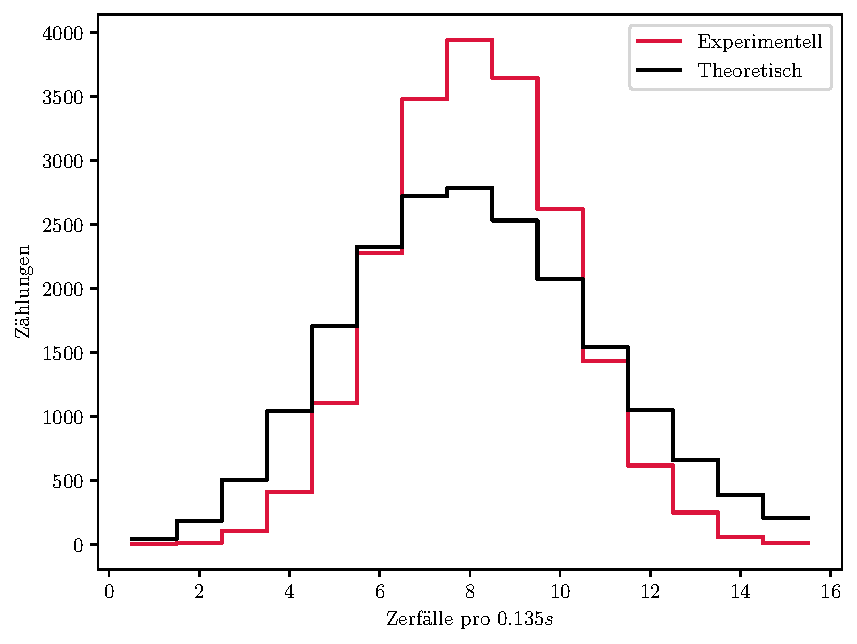
\includegraphics[scale=0.8]{Q7_500V_Poi.pdf}
	\vfill
	\textbf{Abb. 2:}$\quad$Quelle 7 bei 600V: $\lambda=10.0\;,\sigma^2=6.01$
	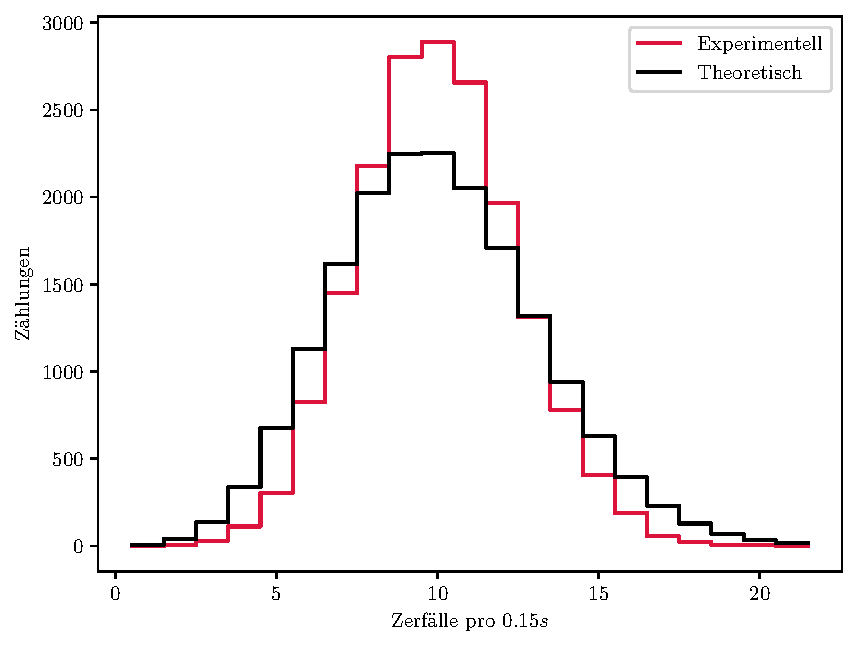
\includegraphics[scale=0.8]{Q7_600V_Poi.pdf}
	\vfill\newpage
	\textbf{Abb. 3:}:$\quad$Quelle 6 \& 7 bei 500V: $\lambda=6.83\;,\sigma^2=2.48$
	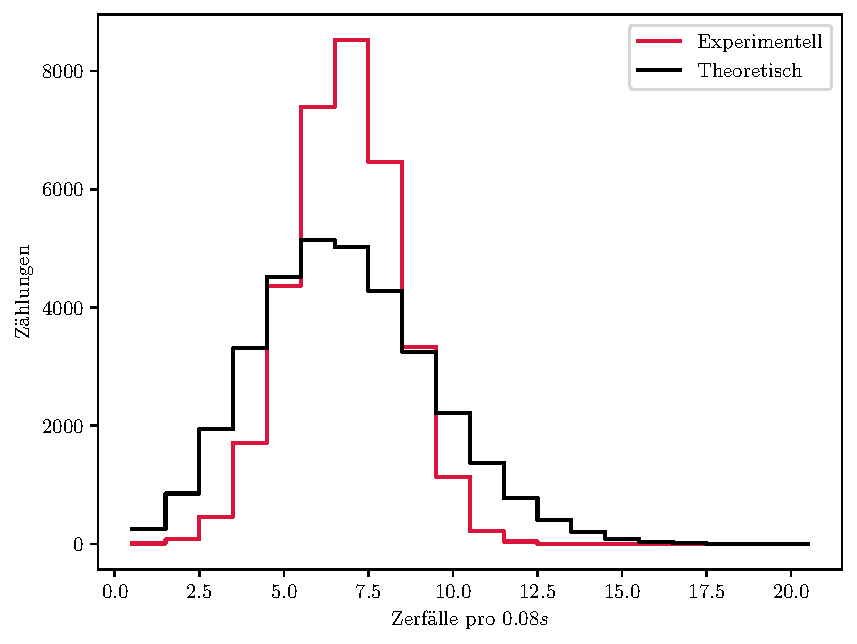
\includegraphics[scale=0.8]{Q67_500V_Poi.pdf}\\
	jdfbsjbfjsdbjfjsb Hier kommen noch coole Vergleiche hin woooow
	\end{center}
	\newpage
	\subsection{Gauß-Verteilung}
	\begin{center}
	\vfill
	\textbf{Abb. 1:}$\quad$Quelle 7 bei 500V: $m=267.17$	
	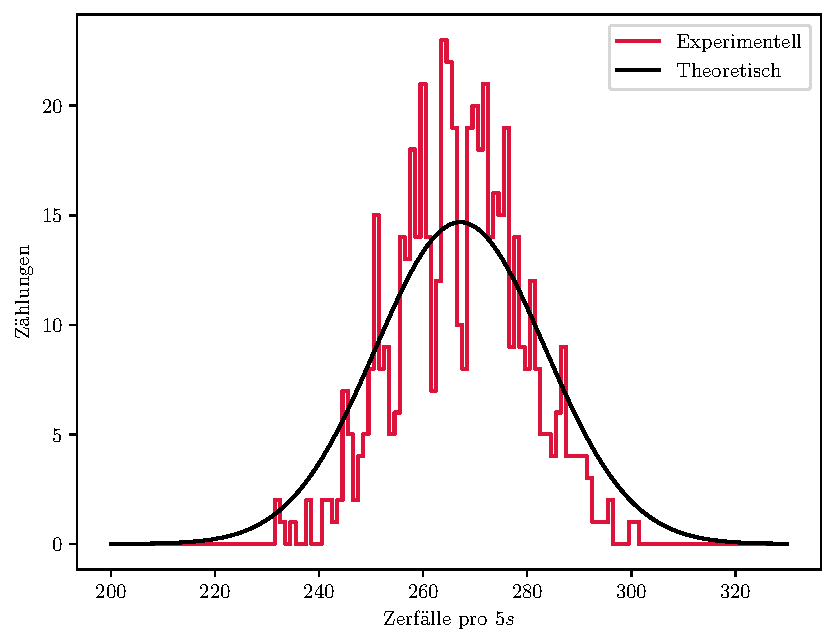
\includegraphics[scale=0.8]{500V_Gauss.pdf}\\
	\vfill
	\textbf{Abb. 2:}$\quad$Quelle 7 bei 600V: $m=301.42$	
	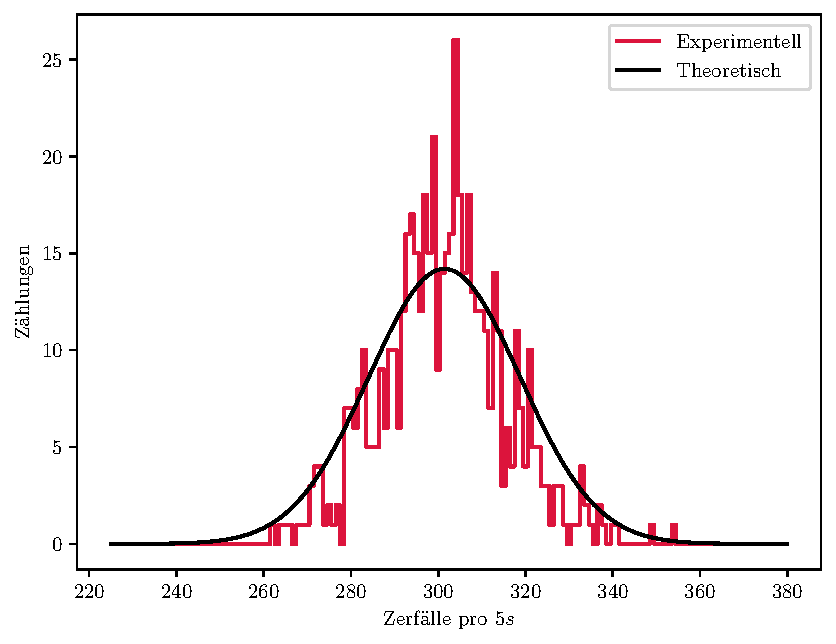
\includegraphics[scale=0.8]{600V_Gauss.pdf}
	\vfill\newpage
	\textbf{Abb. 3:}$\quad$Quelle 6 \& 7 bei 500V: $m=365.08$	
	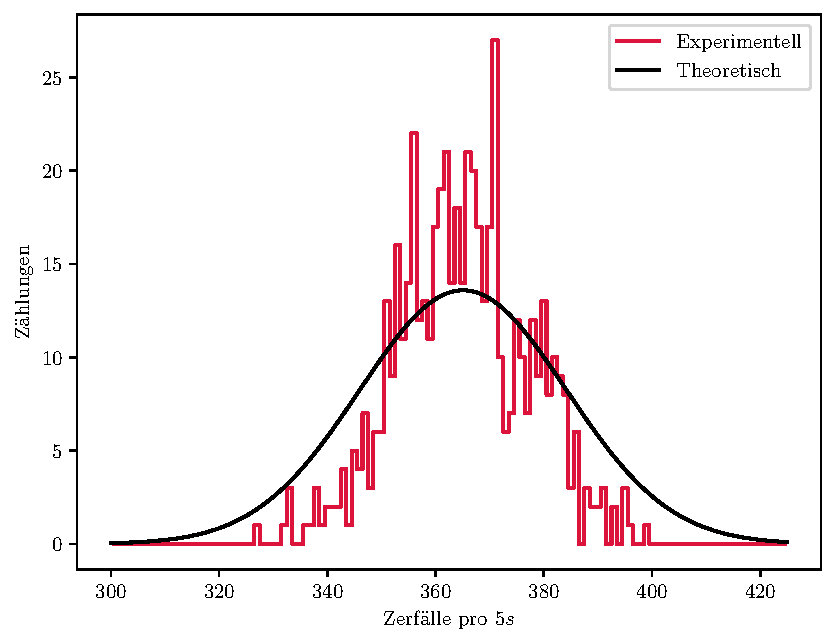
\includegraphics[scale=0.8]{600V_67_Gauss.pdf}\\
	jdfbsjbfjsdbjfjsb Hier kommen noch coole Vergleiche hin woooow
	\end{center}
	\newpage
	\subsection{Intervall-Verteilung}
	\begin{figure}[!h]
	\centering
	\textbf{Abb. 4:}$\quad$Quelle 7 bei 600V
	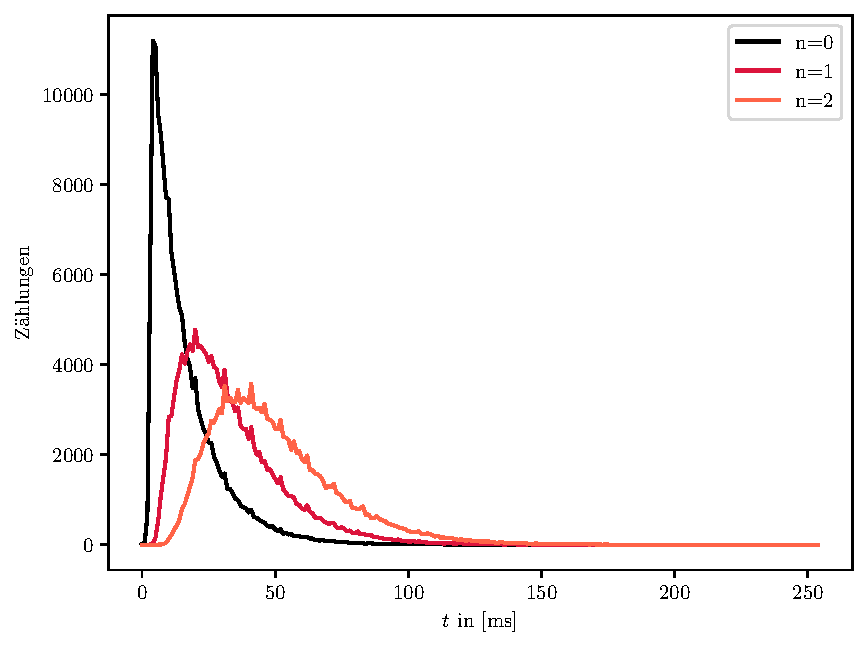
\includegraphics[scale=0.75]{Inter_7_600.pdf}
	\end{figure}\noindent
	Für die Bestimmung des Parameters $a$ einer theoretischen Funktion der Form
	\[P(t)=N\cdot a\cdot e^{-at}\]
	verwenden wir das Julia Paket $LsqFit$\fancyfootnote{Den Code können wir bei Fragen nachsenden.}. Da die ersten 4 Werte der Intervall-Verteilung dem mathematischen Modell nicht genügen wurden diese verworfen, da sie das Ergebnis ungenauer ausfallen lassen.\\
	Man erhält somit einen Fitparameter
	\begin{equation}
	a=(0.0767\pm0.0004)\frac{1}{ms}.
	\end{equation}
	Somit lässt sich die theoretische Funktion gegen die experimentellen Messwerte auftragen:
	\begin{figure}[h!]
		\centering
		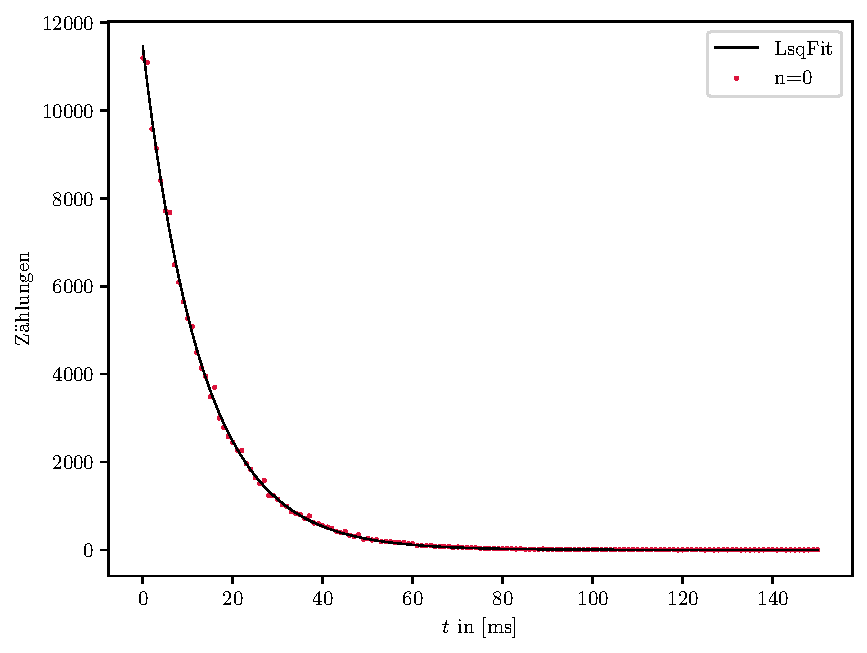
\includegraphics[scale=0.74]{LsqFit.pdf}
	\end{figure}
	\newpage\noindent
	Algorithmisch ist das Anfitten von theoretischen Funktionen an die Messwerte bei $n=1,2$ durchaus möglich, jedoch sind sie stärker von der Totzeit belastet \& man muss zunehmend mehr Messwerte, die das Ergebnis verfälschen, entfernen.\\
	Somit ist es leichter diese über den Fitparameter $a$ bei $n=0$ zu berechnen, wofür man die gegebene Formel umformen kann.
	\begin{gather}
	a=\frac{a'}{1-a'\tau}\;\Leftrightarrow\;\bar{\tau}=\frac{1-\frac{a'}{a}}{a'},\quad a'=\frac{t}{N}\\
	\Delta\tau=\left|\frac{\partial\tau}{\partial a}\Delta a\right|=\frac{1}{a^2}\Delta a\\\notag\\
	\tau=(12.981\pm0.068)ms
	\end{gather}
	\subsection{$\chi^2$-Text}
	Mit dem $\chi^2$-Test prüfen wir nun folgende Hypothesenfür die ersten 51 Messwerte des 10 Sekundenintervalls aus Messung 3:\\
	\begin{enumerate}
	\item Präparatstärkekonstant im betrachteten Zeitraum und gleicht dem Mittelwert der51 Messwerte.
	\item Präparatstärke konstant im betrachteten Zeitraum und gleicht dem Mittelwert der 51 Messwerteminus 10\%.
	\item Präparatstärke nimmt im betrachteten Zeitraum linear mit der Zeit ab (erste Näherung von exp-Abfall) Die Anfangszählrate ist der Mittelwert, und der Abfall von einer Messung zur anderen sei 1.\\
	\end{enumerate}
	
	\noindent
	Für die Hypothese 1) berechnet sich das nicht-totzeitkorrigierte $\chi^2$ wie folgt.\[\chi^2=\sum_{i=1}^{51}\frac{\left(n_i-m\right)^2}{m}\]Um dies totzeit-korrigiert anzugeben benötigt an den Vorfaktor: $\frac{1}{1-\frac{m}{\Delta t}\tau}$ damit folgt gesamt:
	\begin{gather}
	\chi_{kor}^2=\frac{1}{1-\frac{m}{\Delta t}\tau}\cdot\sum_{i=1}^{51}\frac{\left(n_i-m\right)^2}{m}
	\end{gather}
	Wobei $\tau=0,0107s$ die Totzeit des Detektors angibt und $\Delta t$die Länge des gewählten Zeitintervalls angibt ($\Delta t=10s$).Die $n_i$ geben die einzelnen Messwerte an und $m=726,14$ ist der Mittelwert der 51 Messwerte.\\
	Die Hypothese 2) unterscheidet sich nur geringfügig von 1) in dem vom Mittelwert $10\%$ abgezogen wird, also $90\%$ des Mittelwertes $m$. Durch einen einfachen Vorfaktor von $0,9$ beim Mittelwert kann dies sehr leicht erreicht werden. Es gelten die folgenden Formeln für nichtkorrigierte und korrigierte
	
	\begin{gather}
	\chi^2:\chi^2=\sum_{i=1}^{51}\frac{\left(n_i-0.9m\right)^2}{0.9m}\\
	\chi_{kor}^2=\frac{1}{1-\frac{0.9m}{\Delta t}\tau}\cdot\sum_{i=1}^{51}\frac{\left(n_i-0.9m\right)^2}{0.9m}
	\end{gather}
	
	\noindent Um in der Hypothese 3) den gewünschten linearen Abfall zu erreichen, der mit 1 pro Messung skaliert ist, wird von der Anfangszählrate (Mittelwert $m$) bei jedem Schritt 1 abgezogen. So ergeben sich folgende Formeln:
	\begin{gather}
	\chi^2=\sum_{i=1}^{51}\frac{\left(n_i-(m-i)\right)^2}{(m-i)}\\
	\chi_{kor}^2=\sum_{i=1}^{51}{\frac{1}{1-\frac{(m-i)}{\Delta t}\tau}\cdot\frac{\left(n_i-(m-i)\right)^2}{(m-i)}}
	\end{gather}
	\\
	\begin{center}
	\begin{tabular}{|c|c|c|}
		\hline
		Hypothese & $\chi^2$ & $\chi_{kor}^2$\\
		\hline\hline
		1) & $18.38$ & $82.41$\\
		\hline
		2) & $431.90$ & $1436.17$\\
		\hline
		3) & $91.43$ & $350.84$\\
		\hline
	\end{tabular}
	\end{center}
	\noindent
	\\\\Aus der Tabelle im Anhang kann nun abgelesen werden, welche Werte des $\chi^2$-Tests im gewünschten Fehlerbei fester Anzahl von Messwertenliegen. Für einen Fehler von $5\%$ gilt also Werte zwischen $71,4$ ($\chi_{0.975}^2$) und $32,4$ ($\chi_{0.025}^2$) werden angenommen und alle anderen verworfen.\\
	Die Halbwertszeit der Hypothese 3) kann einfach ermittelt werden, da es als linearer Zerfall angenommen wird. Durch die Formel \[\frac{m}{2}=m-\frac{t}{10}\] ermittelt werden. Durch Umformen folgt:
	\begin{equation}
	t=T_\frac{1}{2}=\left(\frac{m}{2}\right)\cdot10
	\end{equation}
	Damit ergibt sich für die Hypothese 3) eine Halbwertszeit von $T_\frac{1}{2}\approx3630.7s$. Dies entspricht etwa einer Stunde. Vergleicht man diese errechnete Halbwertszeit mit dem Literaturwert des $^{137}Cs$ von etwa 30 Jahre, erkennt man, dass das Verwerfen dieser Hypothese durch den $\chi^2$-Test gerechtfertigt ist.
	\subsection{Totzeit}
	\newpage
	\section{Diskussion}
\end{document}